\documentclass[../main.tex]{subfiles}
\graphiscpath{{..figs/}}

\begin{document}
\begin{problema}
	Un oscilador forzado satisface la siguiente ecuación

	\begin{equation}
		\ddot{x} + \Omega^{2}x = F_{0}\cos \biggl[\Omega(1 + \epsilon)t\biggr]
	\end{equation}

	con \(\epsilon\) una constante positiva. Muestra que la solución
	que satisface las condiciones iniciales \(x = 0\) y
	\(\dot{x} = 0\) cuando \(t = 0\) es

	\begin{equation}
		x = \dfrac{F_{0}}{\epsilon \Bigl(1 + \tfrac{1}{2}\Bigr)\Omega^{2}}\sin \Bigl[\tfrac{1}{2}\epsilon\Omega t\Bigr]\sin \Bigl[\Omega(1 + \epsilon)t\Bigr].
	\end{equation}

	Grafica \(x(t)\) cuando \(\epsilon\) es pequeña.
\end{problema}

\startsolution

Tenemos nuevamente u oscilador forzado, cuya solución homogénea es aquella del problema anterior, insert eq., i.e.,

\begin{equation}
	x_{H}(t) =A\cos(\Omega t) + B\sin(\Omega t).
	\label{eq:homogeneous-sol}
\end{equation}

Para calcular la solución particular usamos el método visto en clase. Empezamos escribiendo la \zcref{eq:homogeneous-sol}
como

\begin{equation}
	\ddot{y} + \Omega^{2}y = F_{0}\sin(\Omega(\epsilon + 1)t)
	\label{eq:h-sol-in-y}
\end{equation}

y definimos \(z(t) = x(t) + i y(t)\). Multiplicando la \zcref{eq:h-sol-in-y} por \(i\) y
sumándola a la \zcref{eq:homogeneous-sol},

\begin{equation}
	\ddot{z} + \Omega^{2}z = F_{0}\mathrm{e}^{i\alpha t},
	\label{eq:complex-sol}
\end{equation}

con \(\alpha = \Omega(\epsilon + 1)\). Por lo que la solución tiene la siguiente forma

\begin{align}
	z(t)        & = C \mathrm{e}^{i\alpha t},\label{eq:z-sol}    \\
	\dot{z}(t)  & = Ci\alpha \mathrm{e}^{i\alpha t},\nonumber    \\
	\ddot{z}(t) & = -C\alpha^{2}\mathrm{e}^{i\alpha t}.\nonumber
\end{align}

Entonces, la \zcref{eq:complex-sol} queda como:

\begin{align*}
	(-\alpha^{2} + \Omega^{2})C \mathrm{e}^{i\alpha t} & = F_{0}\mathrm{e}^{i\alpha t},                                  \\
	\Rightarrow C                                      & = \dfrac{F_{0}}{\Omega^{2} - \alpha^{2}},                       \\
	                                                   & = \dfrac{F_{0}}{\Omega^{2} - \Omega^{2}\epsilon(\epsilon + 1)}, \\
	\Aboxedsec{C                                       & = \dfrac{-F^{0}}{\Omega^{2}\epsilon(\epsilon + 1)}.}
\end{align*}

Sustituyendo en la \zcref{eq:z-sol},

\begin{equation*}
	z(t) = \dfrac{-F_{0}}{\Omega^{2}\epsilon(\epsilon + 2)}\mathrm{e}^{i\Omega(\epsilon + 1)}.
\end{equation*}

La solución particular es la parte real de \(z(t)\),

\begin{equation}
	x_{P}(t) = \dfrac{-F_{0}}{\Omega^{2}\epsilon(\epsilon + 2)}\mathrm{e}^{i\Omega(\epsilon + 1)}\cos(\Omega(\epsilon + 1)t).
	\label{eq:particular-sol}
\end{equation}

Sumando las \zcref{eq:homogeneous-sol,eq:particular-sol}, la solución
general es

\begin{equation}
	x(t) = A\cos(\Omega t) + B\sin(\Omega t) - \dfrac{F_{0}}{\Omega^{2}\epsilon(\epsilon + 2)}\cos(\Omega(\epsilon + 1)t).
\end{equation}

Evaluando las condiciones iniciales, \(x(0) = 0 = \dot{x}(0)\),

\begin{align*}
	x(0) = 0                   & = A\cos(0) + B\sin(0) - \dfrac{F_{0}}{\Omega^{2}\epsilon(\epsilon + 2)}\cos(0),              \\
	\Rightarrow\;\Aboxedsec{A  & = \dfrac{F_{0}}{\Omega^{2}\epsilon(\epsilon + 2)},}                                          \\
	\dot{x}(0) = 0             & = -A\Omega\sin(0) + B\Omega\cos(0) - \dfrac{F_{0}}{\Omega^{2}\epsilon(\epsilon + 2)}\sin(0), \\
	\Rightarrow\;\Aboxedsec{ B & = 0.}
\end{align*}

Por lo tanto,

\begin{equation*}
	x(t) = \dfrac{F_{0}}{\Omega^{2}\epsilon(\epsilon + 2)}\cos(\Omega t) - \dfrac{F_{0}}{\Omega^{2}\epsilon(\epsilon + 2)}\cos(\Omega(\epsilon + 1)t).
\end{equation*}

Reescribiendo \(x(t)\),

\begin{equation}
	x(t) = \dfrac{F_{0}}{\Omega^{2}\epsilon(\epsilon + 2)}
	\biggl[\cos(\Omega\epsilon t) - \cos(\Omega(\epsilon + 1)t)\biggr].
\end{equation}

Usando la identidad trigonométrica
\(\cos(\Omega\epsilon t) - \cos(\Omega(\epsilon + 1)t) = -2\sin \bigl[ \tfrac{1}{2}(\Omega(2 + \epsilon)t)\bigr]\sin \bigl[\tfrac{1}{2}(-\Omega\epsilon t)\bigr]\),

\begin{align}
	x(t)             & = \dfrac{F_{0}}{2\epsilon(1 + \tfrac{\epsilon}{2})\Omega^{2}}\Bigl[-2\sin \bigl[ \tfrac{1}{2}(2\Omega(1 + \tfrac{\epsilon}{2})t)\bigr]\bigl[-\sin\bigl[\tfrac{1}{2}(\Omega \epsilon t)\bigr]\bigr]\Bigr],\nonumber \\
	\Aboxedmain{x(t) & = \dfrac{F_{0}}{\epsilon(1 + \tfrac{\epsilon}{2})\Omega^{2}}\sin\bigl[\tfrac{1}{2}\epsilon\Omega t\bigr]\sin \bigl[ \Omega(1 + \tfrac{\epsilon}{2})t\bigr].}\label{eq:complete-sol}
\end{align}

Ahora si \(\epsilon\) es pequeña, la \zcref{eq:complete-sol} queda
como

\begin{align}
	x(t)            & = \dfrac{F_{0}}{\epsilon(1 + \tfrac{\epsilon}{2})\Omega^{2}}\tfrac{1}{2}\epsilon\Omega t\sin(\Omega t),\nonumber \\
	\Aboxedsec{x(t) & = \dfrac{F_{0}}{2\Omega}t\sin(\Omega t).}\label{eq:Approx-sol}
\end{align}

La solución cuando \(\epsilon\) es pequeña da como resultado la
\zcref{ eq:Approx-sol}, cuya gráfica se ve como

\begin{figure}[htb]
	\centering
	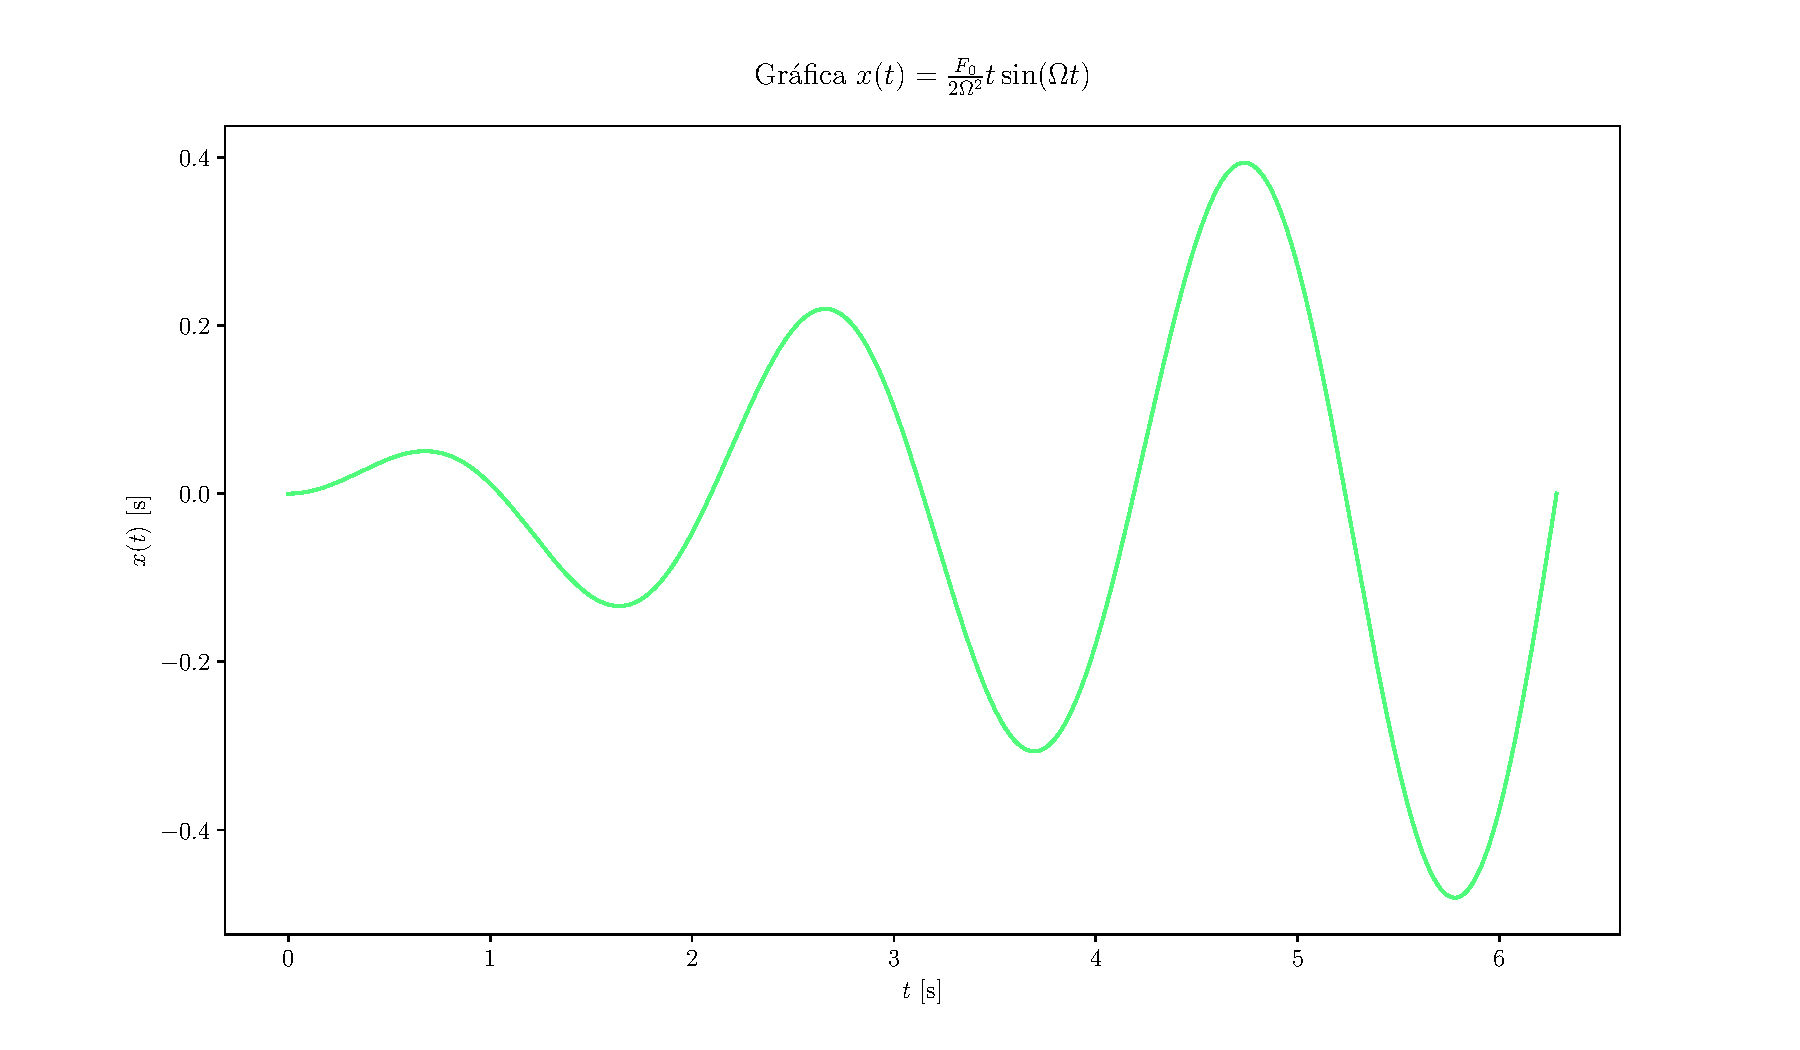
\includegraphics[width=.8\textwidth]{figs/forced-oscillator.pdf}
	\caption{Gráfica de \(x(t)\) para \(F_{0} = 0.5\) y \(\Omega = 3\).}
\end{figure}
\end{document}
